\chapter{Pjproject}\label{cha:pjproject}

\textit{
\begin{quotation}
Tue Aug 14 04:07:02 EDT 2012.
\end{quotation}
\begin{quotation}
I just want to say for everyone, that the Android setup that we support is
what is in https://trac.pjsip.org/repos/wiki/Getting-Started/Android. Even
this setup is experimental as it's currently under development, so expect
some problems.
\end{quotation}
\begin{quotation}
If you decide to use different setup, such as to use the trunk, or to use
pjsua, then YOU ARE ON YOUR OWN. That means you know what you're doing and
you  know how to fix problems yourself. Please don't report any errors or
crashes here as that will only confuse people.
\end{quotation}
}
 \epigraph{ \textit{Best regards, Benny} }
{\textit{Benny Prijono}, Pjproject main developer. \url{http://lists.pjsip.org/pipermail/pjsip\_lists.pjsip.org/2012-August/015136.html}}



\minitoc\mtcskip

\section{Pjproject: descrizione}
Pjproject\syfoot[1]{Chiamerò in questa trattazione il progetto PJSIP 
(\url{http://www.pjsip.org/}) come Pjproject (come tra l'altro indicato dal
nome del \textit{trunk} del sorgente (\url{http://svn.pjsip.org/repos/}), per non
confonderlo confonderlo con la stessa libreria \texttt{pjsip} presente all'interno
dello stesso progetto.} è una libreria scritta in linguaggio C adoperata allo
scopo di implementare il protocollo di comunicazione SIP. La struttura di 
questo progetto è inoltre mirata a garantire un'estrema configurabilità ed 
indipendenza dal sistema operativo nel quale tale libreria verrà utilizzata.
Allo scopo viene predisposto un primo strato, definito dalla sottolibreria \texttt{\small pj},
nel quale vengono fornite le implementazione delle funzioni basilari che verranno
utilizzate, più o meno direttamente, da tutti gli altri strati rappresentati dalle
sottolibrerie fornite dal progetto di Pjproject. Oltre alla libreria \texttt{\small pjmedia}
di cui parlerò per la gestione dei file(s) multimediali, utilizzerò nella seguente
trattazione la libreria \texttt{\small pjsua}, che implementa un livello di
astrazione, allo scopo di 
realizzare applicazioni utente di alto livello. Questa consente di \parencite{man:pjsip}:
\begin{itemize}
\item Effettuare la registrazione di utenti e loro gestione.
\item Supportare chiamate concorrenti.
\item Gestione dello stato delle chiamate.
\item Supporto wideband delle informazioni multimediali, supporto di codec audio
	e di riproduzione di file multimediali.
\end{itemize}

\begin{figure}[thp]
\centering
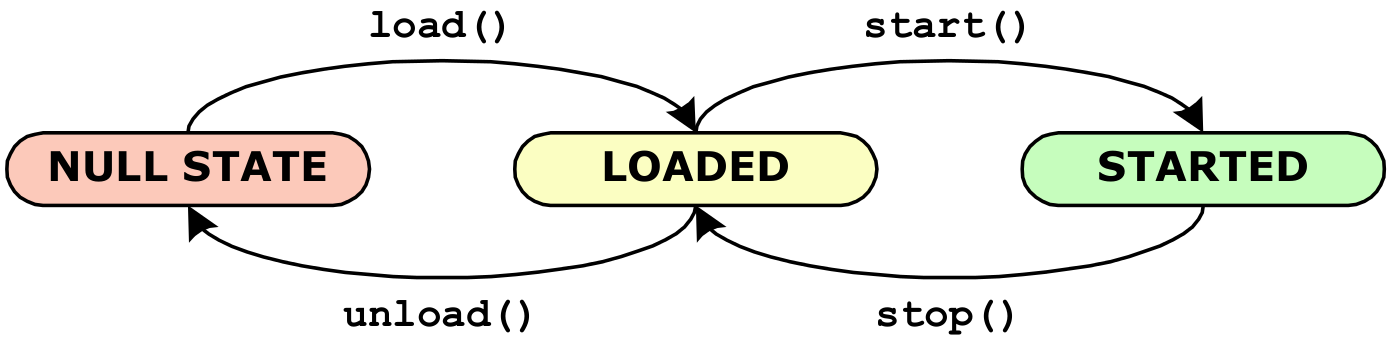
\includegraphics[scale=0.3]{img/libraries/modulestatepjsip.png}
\caption{\textit{Diagramma degli stati di un modulo}.\parencite{man:pjsip}}
\label{fig:pjprojectmod}
\end{figure}

Questa libreria è inoltre strutturata sulla gestione di moduli, i quali hanno
lo scopo di distribuire i messaggi SIP tra i vari strati, e di implementare
un'interfaccia di astrazione. Questi moduli, come illustrato in Figura
\vref{fig:pjprojectmod}, sono caratterizzati da stati che mostrano lo stato
di attività degli stessi. Questi sono gestiti da un \texttt{pjsip\_endpoint}, il 
quale si preoccupa di far transitare i messaggi tra i moduli o di attivarne
i callback in base al loro grado di priorità, definito in base alla loro posizione
all'interno dello stack dei moduli e delle corrispondenti librerie.
\medskip

Descriverò ora quale sia la struttura di un device audio all'interno di Pjproject:
faccio riferimento allo stesso sorgente di \texttt{\small pjsua},
ottenibile all'interno del sorgente del \textit{branch} per Android\footnote{Nota:
questo branch è ritenuto, al momento di redazione della tesi, ancora instabile.
Tuttavia non sono stati in questo caso risolti i problemi posti in precedenza,
tra cui i flag di compilazione. Sorgente: \url{http://svn.pjsip.org/repos/pjproject/branches/projects/android/}.}.
In quanto non è disponibile una spiegazione maggiormente dettagliata del codice
sorgente stesso, per spiegare come avvenga questo meccanismo, debbo far riferimento
al codice presente in
\begin{center}
\texttt{\small \PJA/pjsip-apps/src/pjsua}
\end{center}
dove con \texttt{\small \PJA} indico il percorso dove sono situati i sorgenti di 
tale \textit{branch}. 

Ogni modulo della libreria fornisce un accesso compatto alle funzioni definite
all'interno del file sorgente: questo consente di fornire un'unica interfaccia a tutti 
i moduli di una stessa tipologia, che possono quindi essere implementati differentemente
in base ai singoli obiettivi di realizzazione. Questo discorso è estendibile a tutti
i device implementati all'interno del percorso:
\begin{center}
\texttt{\small \PJA/pjmedia/src/pjmedia-audiodev}
\end{center}
Soffermandomi in particolare sul file \texttt{\small opensl\_dev.c} dov'è presente
l'implementazione dell'interazione con la scheda audio tramite libreria
\texttt{\small wilhelm}, posso notare come sia predisposta una factory 
allo scopo di fornire una pool per l'allocazione dei dati, il riferimento
all'\textit{engine} OpenSL ES ed una serie di funzioni per gestire lo stream di
dati.

Quando farò riferimento alla versione \textit{trunk},
mi riferirò alla versione 2.0, ottenibile
al seguente indirizzo:
\url{http://www.pjsip.org/release/2.0/pjproject-2.0.tar.bz2}

\section{Premesse al porting di Pjproject}




\subsection{Definizione di \texttt{user.mak}}
Questo è il file preposto dagli sviluppatori di Pjproject allo scopo di definire
dei flag necessari allo sviluppatore. Ne forniamo di seguito l'implementazione:

\lstinputlisting[language=bash,caption= user.mak]{srcs/user.mak}

In particolare si è ritenuto necessario specificare l'oggetto \texttt{\small /path/to/crt0.o},
in quanto si riscontrano problemi che possono
insorgere dalla sua mancata definizione e quindi dalla mancata invocazione
dell'inizializzazione della libreria \textit{Bionic}. In particolare in fase di compilazione
è possibile osservare il seguente avvertimento:
\begin{center}
\texttt{\small : warning: cannot find entry symbol \_start; defaulting to 00008280}
\end{center}
In mancanza della definizione di \texttt{\small \_start} verrà utilizzata, come 
funzione sostituta, una presente nel  programma che si sta crosscompilando.
Nel caso di \texttt{\small pjsua} la prima funzione coincideva con quella di main
e quindi, in completa assenza di tale binario, il programma partiva (apparentemente) correttamente, ma visualizzando il
seguente output.
\begin{bash}
21:37:35.213 os_core_unix.c !pjlib 2.0 for POSIX initialized
21:37:35.229 sip_endpoint.c  .Creating endpoint instance...
21:37:35.233          pjlib  .select() I/O Queue created (0x168c7c)
21:37:35.236 sip_endpoint.c  .Module "mod-msg-print" registered
21:37:35.236 sip_transport.  .Transport manager created.
21:37:35.236   pjsua_core.c  .PJSUA state changed: NULL --> CREATED
Segmentation Fault
\end{bash}
In particolare il LogCat evidenzia l'evoluzione delle chiamate a funzione
tramite il tracciamento dei valori assunti dallo stackpointer:
\begin{bash}
I/DEBUG   (   96):          #00  pc 00093ea8  /data/local/bin/pjsua (_getopt_internal.constprop.1)
I/DEBUG   (   96):          #01  pc 0001282c  /data/local/bin/pjsua (app_init)
I/DEBUG   (   96):          #02  pc 0000bbbc  /data/local/bin/pjsua (main_func)
I/DEBUG   (   96):          #03  pc 000b4b5c  /data/local/bin/pjsua (pj_run_app)
\end{bash}
Nella prima funzione avviene il parsing dei parametri, che termina
con un \textit{Segmentation Fault} in quanto si tenta di raggiungere un argomento che ha
valore \texttt{NULL}. La definizione della funzione \texttt{\_start} e la conseguente
chiamata all'inizializzazione di suddetta libreria porta al superamento dell'ostacolo
sopra descritto.


\subsection{Definizione di \texttt{configure-android} e \texttt{myConf}}
Questo primo script è stato proposto all'interno del branch Android di Pjproject, che
riporto all'interno del Listato \vref{alg:confandroid}. In particolare
utilizzo la versione 4.6 della toolchain di cross-compilazione,
e specifico in \texttt{\small LDFLAGS} il parametro \texttt{\small -nostdlib} per
forzare l'utilizzo delle librerie incluse nel percorso indicato dal flag \texttt{\small -L}.

\begin{algorithm}[thp]
\lstinputlisting[language=bash,caption=$ $configure-android,label=alg:confandroid]{srcs/configure-android}
\end{algorithm}

Lo script precedente viene lanciato dal seguente:
\lstinputlisting[language=bash,caption= myConf]{srcs/myConf}
in questo caso definisco le variabili d'ambiente per  il percorso base
dell'NDK, il numero dell'API Android per la quale effettuare la compilazione,
la riconfigurazione dell'\texttt{\small aconfigure.ac} in seguito al patching,
la definizione del file
\begin{center}
\texttt{\small pjlib/include/pj/config\_site.h}
\end{center}
per la definizione personalizzata dei flag di inclusione, e la disabilitazione
del linking dei moduli di pjsua per i codec non supportati da Android.

In particolare posso effettuare le seguenti osservazioni:
\begin{itemize}
\item Oltre all'inclusione della libreria \texttt{\small -lc}, è necessario includere
	anche \texttt{\small -lgcc} in quanto altrimenti non si troverà \texttt{\small\_start}
\item Per effettuare il linking tra codice C e C++ è necessario specificare
	l'opzione \texttt{\small -fno-exceptions}, in quanto le eccezioni non si
	devono propagare da C++ a C.
\item Per poter effettuare il linking con la libreria audio di Android, si specifica
	l'opzione \texttt{\small -lOpenSLES}.
\end{itemize}
